
\chapter{Introduction}

% 학위논문 주제 설정의 배경, 관련 분야에서 기존의 연구,
% 본 논문의 취지, 실험 논문의 경우 연구에 대한 간략한 소개와
% 연구를 위해 설정한 가설 등을 소개한다.

\section{Sequence Databases}

Next generation sequencing (NGS) technologies have revolutionized the way we collect and analyze biological data. Thanks to NGS, the cost of sequencing has dropped drastically and continued to decrease with more new technologies developed. Accompanying this change is the explosive growth of the amount of sequencing data and the size of sequence databases. The Sequence Read Archive (SRA) is one of the most popular and widely used sequence databases that store both private and public sequence reads and provide access in various foramts including the commonly used \texttt{FASTQ} file format. Its size has grown exponentially since 2008 and currently reached more than 60 petabytes large. The growth in size of Sequence Read Archive is visualized in \autoref{fig:sra_stat}.



\section{State-of-the-art Algorithms for Sequence Searches}

\subsection{DIAMOND}

\subsection{MMseqs2}

\subsection{BIGSI}

\section{Prototype of Petasearch Algorithm}

\section{Motivation and Contribution of the Thesis}

The search of homologs in large sequence databases requires a fast yet sensitive enough algorithm specially designed for petabyte-scale analysis. The state-of-the-art searching algorithms failed to satisfy this need. The prototype of \texttt{Petasearch}, despite its idea proven to be promising, has not reached its peak speed efficiency and is rather heavy in disk consumption. Limited by the current design, its searching sensitivity is also less desirable for homologs with sequence similarity less than 40\%. To tackle these problems and make \texttt{Petasearch} more available to the public, we revised the design of the core data structures of \texttt{Petasearch} and added the profile-search functionality. The main contribution of this thesis is the major improvement of the \texttt{Petasearch} algorithm in speed, space consumption and sensitivity.

In chapter 2, we will continue with describing the further development and optimization of \texttt{Petasearch}. We will also describe the design of the benchmarks in chapter 2. In chapter 3, we will first show the improvements in efficiency and effectiveness of the forementioned optimizations. Afterwards, we will show a thorough comparison of the performance of the \texttt{Petasearch} algorithm with the state-of-the-art algorithms. In chapter 4, we will discuss the potential application of \texttt{Petasearch} and show two examples of its usage.

\pagebreak

\begin{figpage}
\begin{figure}[t]
  \centering
  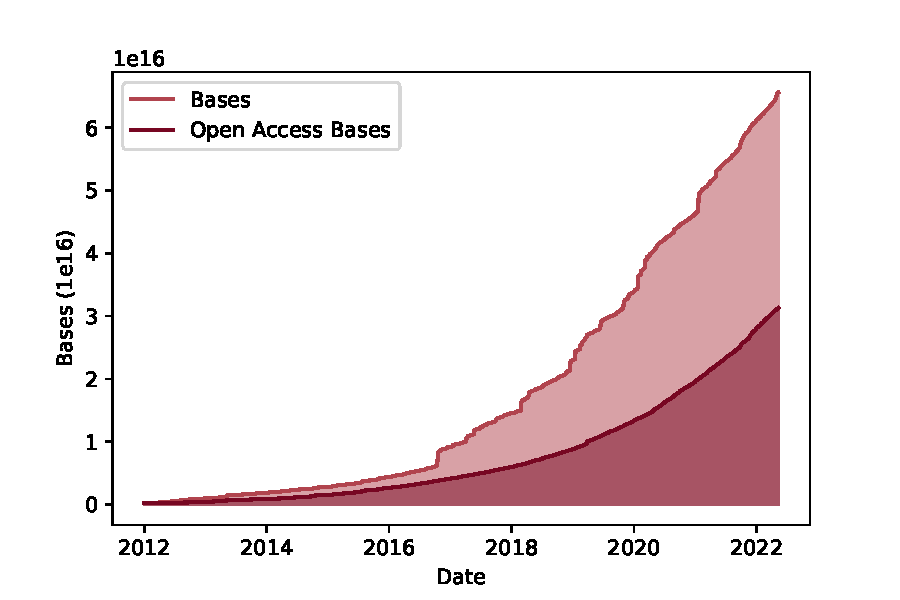
\includegraphics[width=\textwidth]{images/sra_stat.pdf}
  \caption{The exponential growth of the Sequence Read Archive from 2008 to 2022. The total amount of sequence data (unit in bases) and publicly available data are visualized in pink and dark red respectively.}
  \label{fig:sra_stat}
\end{figure}
\end{figpage}
